\chapter{The OSI Model}\label{sec:osi_intro}
\section{What is OSI?}
\begin{figure}[h]
    \centering
    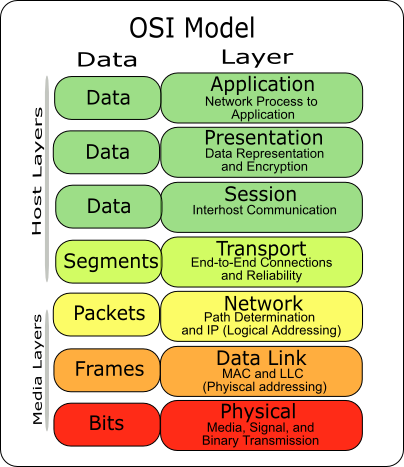
\includegraphics[width=.6\textwidth]{assets/osi/layers.png}
    \caption{The OSI Model Layers}\label{fig:osi_layers_intro}
\end{figure}
From chaos to order, the Open Systems Interconnection (OSI) model is a framework we use to understand how different networking protocols interact. Coincidentally (not so much), the Computer Networks course is structured around it.

You don't need to memorize these layers right off the bat, as, instead of that, we would like for you to understand each layer's purpose \textit{before} knowing the correct term for it. That way, you will be able to come up with the term yourself!

\section{Why OSI? $\star$}
The development of the model began in the late 1970s as a collaborative effort to standardize networking (See Figure \ref{fig:standards}). The model emerged from the need to connect networking systems that were using proprietary protocols from vendors like IBM and DEC.

\vspace{1em}
\begin{figure}[h]
    \centering
    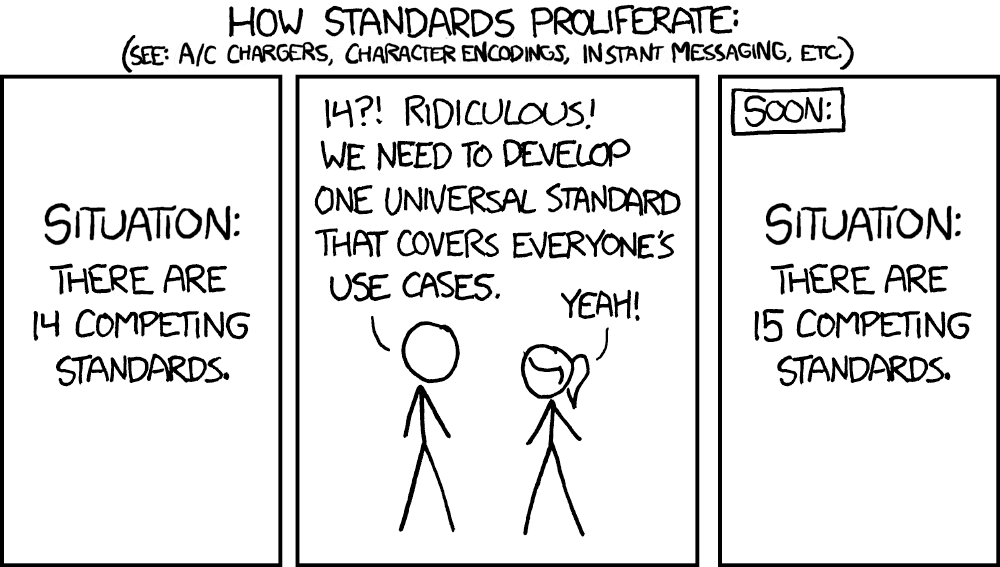
\includegraphics[width=.6\textwidth]{assets/osi/physical/standards.png}
    \caption{XKCD \#927: \href{https://xkcd.com/927/}{Standards}}
    \label{fig:standards}
\end{figure}

The OSI model was formally defined in 1978 by Hubert Zimmermann and published as an ISO\footnote{
    You're going to be seeing this acronym a lot, so let's get it out of the way: ISO stands for International Organization for Standardization.
} standard in 1984. Despite its comprehensive framework, it ultimately lost to the simpler TCP/IP model (Figure \ref{fig:osi_vs_tcpip}), which during the `Protocol Wars' of the 1980s and 1990s. Nonetheless, the OSI model remains a valuable tool for understanding networking concepts and protocols.

\begin{figure}[h]
    \centering
    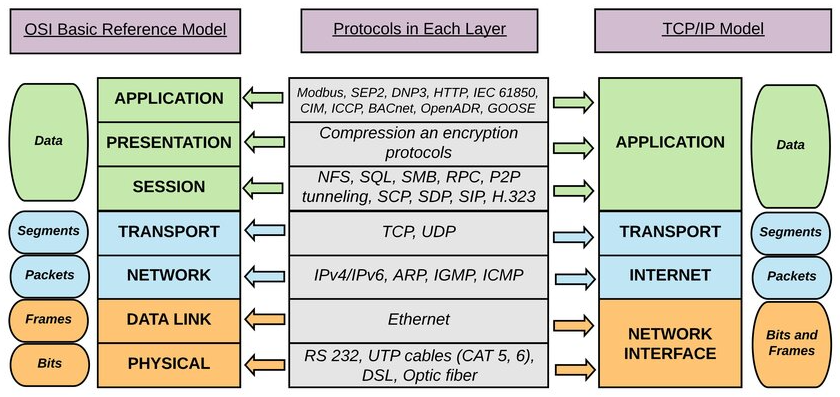
\includegraphics[width=.7\textwidth]{assets/osi/physical/tcp_vs_osi.png}
    \caption{OSI vs TCP/IP}
    \label{fig:osi_vs_tcpip}
\end{figure}






